\documentclass[a4paper]{article}

\SweaveOpts{keep.source=TRUE}
%\VignetteIndexEntry{Detailed introduction to all major features of BoolNet}

\usepackage{a4wide}

\usepackage{graphicx}
\usepackage{amsmath}
\usepackage{hyperref}

\usepackage{listings}
\lstset{breaklines=true, breakautoindent=false, breakindent=0pt, columns=fullflexible,keepspaces=true, basicstyle=\small\ttfamily}

\setlength{\parindent}{0em}
\setlength{\parskip}{0.2em}

\title{BoolNet package vignette}
\author{Christoph M\"ussel, Martin Hopfensitz, Hans A. Kestler}

\widowpenalty=10000
\clubpenalty=10000

\hyphenation{me-thods pro-per-ties re-pre-sen-ta-tion}

\begin{document}
\SweaveOpts{concordance=TRUE}
\maketitle
\tableofcontents

\clearpage
\section{Introduction}

\texttt{BoolNet} is an R package that provides tools for assembling, analyzing and visualizing synchronous and asynchronous Boolean networks as well as probabilistic Boolean networks. This document gives an introduction to the usage of the software and includes examples for use cases.

\texttt{BoolNet} supports four types of networks:
\begin{description}
\item[Synchronous Boolean networks]{ consist of a set of Boolean variables 
\[
X = \left\{X_1, \ldots, X_n \right\} 
\]
and a set of transition functions 
\[
F=\left\{ f_{1},\ldots,f_{n}\right\},
\] 
one for each variable. These transition functions map an input of the Boolean variables in $X$ to a Boolean value ($0$ or $1$). We call a Boolean vector $\mathbf{x}(t) = \left(x_1(t), \ldots, x_n(t) \right)$ the {\em state} of the network at time $t$. Then, the next state of the network  $\mathbf{x}(t)$ is calculated by applying {\em all} transition functions $f_i(\mathbf{x}(t-1))$.

In a biological context, genes can be modeled as Boolean variables ({\em active/expressed} or {\em inactive/not expressed}), and the transition functions model the dependencies among these genes. In the synchronous model, the assumption is that all genes are updated at the same time. This simplification facilitates the analysis of the networks.}

\item[Asynchronous Boolean networks]{ have the same structure as synchronous Boolean networks. Yet, at each point of time $t$, only {\em one} of the transition functions $f_i \in F$ is chosen at random, and the corresponding Boolean variable is updated. This corresponds to the assumption that in a genetic network, gene expression levels are likely to change at different points of time. In the most common model, the gene to be updated is chosen uniformly among all genes. Moreover, \texttt{BoolNet} supports specifying non-uniform update probabilities for the genes.}

\item[Probabilistic Boolean networks (PBN)]{ allow for specifying more than one transition function per variable/gene. Each of these functions has a probability to be chosen, where the probabilities of all functions for one variable sum up to 1. Formally
\[
F=\left\{\left\{\left(f_{11}, p_{11}\right), \ldots, \left(f_{1k_1}, p_{1k_1}\right)\right\}, \ldots,  \left\{\left(f_{n1}, p_{n1}\right), \ldots, \left(f_{nk_n}, p_{nk_n}\right)\right\}\right\}
\]

where $k_i$ is the number of alternative transition functions for variable $i$, and $p_{ij}$ is the probability that function $j$ is chosen for variable $i$. A state transition is performed by selecting one function for each gene based on the probabilities and applying the chosen functions synchronously.}

\item[Temporal Boolean networks]{ are Boolean networks that incorporate temporal predicates and discrete time delays. Here, the next state $x(t)$ may not only depend on $x(t-1)$, but can depend on any predecessor state $x(t - \Delta), \Delta \in \{1, 2, \ldots\}$. Furthermore, $x(t)$ may also directly depend on the time step $t$ itself.
}

\end{description}

In \texttt{BoolNet}, there are different structure classes representing these network types:
\begin{description}
\item[\emph{BooleanNetwork} objects]{ contain synchronous and asynchronous Boolean networks. Here, the transition functions are internally represented as truth tables.}
\item[\emph{ProbabilisticBooleanNetwork} objects]{ encode Probabilistic Boolean networks. They use a truth table representation as well.}
\item[\emph{SymbolicBooleanNetwork} objects]{ represent synchronous and temporal Boolean networks. They encode Boolean functions in a symbolic form, i.e. as expression trees.}
\end{description}
As we have seen, the networks are represented in two different forms: The truth table representation, which basically maps inputs to the corresponding output values, is usually the most efficient representation for synchronous, asynchronous and probabilistic networks and uses a very fast simulator. However, this representation grows exponentially with the number of inputs and is therefore inappropriate for networks with a high number of inputs. This is particularly the case for temporal networks, where each unique time delay for a gene encodes an input. Hence, temporal networks are represented by directly encoding the corresponding Boolean expressions and use a different simulator. As synchronous Boolean networks are a special case of temporal networks (with all time delays being 1), these networks can also be represented as \emph{SymbolicBooleanNetwork} objects.

The package provides several methods of constructing networks:
Networks can be loaded from files in which human experts describe the dependencies between the genes. Furthermore, they can be reconstructed from time series of gene expression measurements. It is also possible to generate random networks. This can be helpful for the identification of distinct properties of biological networks by comparison to random structures. The different methods of assembling networks are described in Section~\ref{sec:assemblingnetworks}.

In Section~\ref{sec:networkanalysis}, tools for the analysis and visualization of network properties are introduced. For synchronous, asynchronous and temporal Boolean networks, the most important tool is the identification of attractors. Attractors are cycles of states and are assumed to be associated with the stable states of cell function. 
Another possibility of identifying relevant states is the included Markov chain simulation. This method is particularly suited for probabilistic networks and calculates the probability that a state is reached after a certain number of iterations. To test the robustness of structural properties of the networks to noise and mismeasurements, the software also includes extensive support for perturbing networks. In this way, it is possible to test these properties in noisy copies of a biological network.

In Section~\ref{sec:importexport}, the interaction of \texttt{BoolNet} with related software is described. In particular, the import from and export to SBML is discussed. Also, the necessary steps to import networks import networks from BioTapestry and to export networks to Pajek are outlined. 

For the examples in the following sections, we assume that the \texttt{BoolNet} package has been properly installed into the R environment. This can be done by typing
\begin{knitrout}
\definecolor{shadecolor}{rgb}{0.969, 0.969, 0.969}\color{fgcolor}\begin{kframe}
\begin{alltt}
\hlkwd{install.packages}\hlstd{(}\hlstr{"BoolNet"}\hlstd{)}
\end{alltt}
\end{kframe}
\end{knitrout}
into the R console or by the corresponding menu entries in an R GUI. For some of the plots, the \texttt{igraph} package is required and must be installed in your R environment as well. This is analogous to installing \texttt{BoolNet}. For the BioTapestry and SBML import, the \texttt{XML} package must be installed.
After installation, the \texttt{BoolNet} package can be loaded via
\begin{knitrout}
\definecolor{shadecolor}{rgb}{0.969, 0.969, 0.969}\color{fgcolor}\begin{kframe}
\begin{alltt}
\hlkwd{library}\hlstd{(BoolNet)}
\end{alltt}
\end{kframe}
\end{knitrout}


\section{Assembling networks}\label{sec:assemblingnetworks}

\subsection{Assembling a network from expert knowledge}

A major advantage of Boolean networks is the fact that natural-language statements can easily be transferred into this representation. This allows researchers for building Boolean networks entirely from expert knowledge, for example by collecting statements on gene dependencies from literature and expressing them as Boolean rules. 

\texttt{BoolNet} is able to read in networks consisting of such rule sets in a standardized text file format. In such a file, each line consists of a target gene and an update rule, usually separated by a comma. Optionally, it is also possible to add a probability for the rule if the file describes a probabilistic network. The first line of such a file is a header

\begin{samepage}
\begin{verbatim}
targets, factors
\end{verbatim}

or

\begin{verbatim}
targets, factors, probabilities
\end{verbatim}
\end{samepage}

To illustrate the process of transforming natural-language statements into Boolean rules, we take a look at the mammalian cell cycle network introduced by Faur\'e et al. \cite{faure06}.  In Table 1 of this paper, the authors list natural-language statements of gene dependencies and the corresponding Boolean expressions. The following rules are taken from this table.

For gene CycD, Faur\'e et al. state:
\begin{quote}
\textit{CycD is an input, considered as constant.}
\end{quote}
Transforming this into a Boolean rule is rather simple: CycD does not change its value, which means that its value after a transition only depends on its previous value. Thus, the transition rule is

\begin{verbatim}
CycD, CycD
\end{verbatim} 
 
 Gene Rb has a more complex description:
 
 \begin{quote}
 \textit{Rb is expressed in the absence of the cyclins, which inhibit it by phosphorylation [...]; it can be expressed in the presence of CycE or CycA if their
inhibitory activity is blocked by p27.} 
 \end{quote}
 
 As a general rule, inhibition can be represented by a Boolean negation. In the \texttt{BoolNet} file format, a negation is expressed by the \texttt{!} character. The referenced cyclins comprise the genes CycA, CycB, CycD, and CycE. If {\em all} these genes are absent, Rb is expressed -- i.e. if CycA is not expressed {\em and} CycB is not expressed {\em and} CycD is not expressed {\em and} CycE is not expressed. A logical AND is embodied by the \texttt{\&} character. Consequently, the first part of the rule is
 \begin{verbatim}
 ! CycA & ! CycB & ! CycD & ! CycE
 \end{verbatim}
In combination with the above statement, the fact that Rb can be expressed in the presence of CycE and CycA if p27 is active means that CycB and CycD must not be active. Thus, the second part of the rule is
\begin{verbatim}
p27 & ! CycB & ! CycD 
\end{verbatim}
This statement is an exception (or alternative) to the first statement; this can be expressed as a logical OR, for which the \texttt{|} character is used.

The complete rule for gene Rb is thus
\begin{verbatim}
Rb, (! CycA & ! CycB & ! CycD & ! CycE) | (p27 & ! CycB & ! CycD)
\end{verbatim}

After processing all genes in the table in this way, we get the following network description:

\begin{samepage}
\begin{footnotesize}
\begin{verbatim}
targets, factors
CycD, CycD
Rb, (! CycA & ! CycB & ! CycD & ! CycE) | (p27 & ! CycB & ! CycD)
E2F, (! Rb & ! CycA & ! CycB) | (p27 & ! Rb & ! CycB)
CycE, (E2F & ! Rb)
CycA, (E2F & ! Rb & ! Cdc20 & ! (Cdh1 & UbcH10)) | (CycA & ! Rb & ! Cdc20 & ! (Cdh1 & UbcH10))
p27, (! CycD & ! CycE & ! CycA & ! CycB) | (p27 & ! (CycE & CycA) & ! CycB &! CycD)
Cdc20, CycB
Cdh1,(! CycA & ! CycB) | (Cdc20) | (p27 & ! CycB)
UbcH10, ! Cdh1 | (Cdh1 & UbcH10 & (Cdc20 | CycA | CycB))
CycB, ! Cdc20 & ! Cdh1
\end{verbatim} 
\end{footnotesize}
\end{samepage}

Now save this description to a file ``cellcycle.txt'' in your R working directory. The network can be loaded via
\begin{knitrout}
\definecolor{shadecolor}{rgb}{0.969, 0.969, 0.969}\color{fgcolor}\begin{kframe}
\begin{alltt}
\hlstd{cellcycle} \hlkwb{<-} \hlkwd{loadNetwork}\hlstd{(}\hlstr{"cellcycle.txt"}\hlstd{)}
\end{alltt}
\end{kframe}
\end{knitrout}
The result is an object of class \emph{BooleanNetwork} containing a truth table representation of the network. 

The same network is also included in \texttt{BoolNet} as an example and can be accessed via
\begin{knitrout}
\definecolor{shadecolor}{rgb}{0.969, 0.969, 0.969}\color{fgcolor}\begin{kframe}
\begin{alltt}
\hlkwd{data}\hlstd{(cellcycle)}
\end{alltt}
\end{kframe}
\end{knitrout}

\texttt{BoolNet} also provides several convenience operators that can be used to express complex Boolean functions in a compact way, e.g.
\begin{itemize}
\item \texttt{maj(a, b, ...)} is 1 if the majority of its operands are 1. Similarly, \texttt{sumgt(a, b, ..., N)} is 1 if more than $N$ operands are 1, \texttt{sumlt(a, b, ..., N)} is 1 if less than $N$ operands are~1, and \texttt{sumis(a, b, ..., N)}  is 1 if exactly $N$ operands are 1.
\item \texttt{all(a, b, ...)} is 1 if all its operands are 1 (i.e. a logical AND), and \texttt{any(a, b, ...)} is~1 if at least one of its operands is 1 (i.e. a logical OR).
\end{itemize}

The cell cycle network is a classical Boolean network, where each transition function only depends on the previous state of the network. E.g., \verb+CycB, ! Cdc20 & ! Cdh1+ can be written formally as $CycB(t) = \neg Cdc20(t-1)  \wedge \neg Cdh1(t-1)$. As already discussed before, \texttt{BoolNet} also incorporates several temporal extensions. For example, a transition function can also depend on the states of genes at earlier time points:
\begin{verbatim}
a, b[-3] & b[-2] & b
\end{verbatim}
is 1 if b has been active in the previous three time steps. The operators described above can also incorporate time ranges. The previous statement can be written in a more compact way using the \texttt{all} operator:
\begin{verbatim}
a, all[d=-3..-1](b[d])
\end{verbatim}
This defines a time delay variable \texttt{d} that can be used for time specifications inside the operator. It can also be used in arithmetic operations. E.g.,
\begin{verbatim}
a, all[d=-3..-1](b[d] & c[d-1])
\end{verbatim}
specifies that a is active if b has been active in the previous three time steps and c has been active at time $t-4$, $t-3$ and $t-2$. 

Apart from relative time specifications, the \texttt{BoolNet} network language also incorporates predicates that depend on the absolute time, i.e. the number of time steps that have elapsed since the initial state. 

\begin{samepage}
For example,
\begin{verbatim}
a, timeis(3)
\end{verbatim}
specifies that \texttt{a} is active at time step 3 and inactive at all other time steps. Similarly, the predicates \texttt{timelt} and \texttt{timegt} evaluate to 1 before and after the specified time point respectively.
\end{samepage}

As the above examples do not cover all possibilities of the network description language, a full language specification is provided in Section~\ref{sec:appendix}.

For temporal networks, \texttt{BoolNet} uses a special symbolic simulator that represents the functions as expression trees, whereas the standard simulator is based on a truth table representation. These simulators are discussed in Section~\ref{sec:networkanalysis}. As synchronous Boolean networks are a special case of temporal networks, they can also be simulated with the symbolic simulator. When a network is loaded from a file using \texttt{loadNetwork()}, the user can specify the parameter \texttt{symbolic=TRUE} to load it in form of a \emph{SymbolicBooleanNetwork} object instead of a \emph{BooleanNetwork} object. The same parameter is also available for the import functions discussed in Section~\ref{sec:importexport}. Temporal networks can only be loaded with \texttt{symbolic=TRUE}, as \texttt{BoolNet} cannot represent them as truth tables.

\begin{sloppypar}
As many network generation and modification routines (such as random network generation and network reconstruction that are discussed in the following sections) internally use the truth table representation, there are conversion routines \texttt{truthTableToSymbolic()} and \texttt{symbolicToTruthTable()} that convert synchronous Boolean networks of class \emph{BooleanNetwork} in a truth table representation to networks of class \emph{SymbolicBooleanNetwork} in a symbolic representation and vice versa. For more details, please refer to the manual.
\end{sloppypar}

\subsection{Reconstructing a network from time series}

An entirely different approach of assembling a network is to infer rules from series of expression measurements of the involved genes over time. For example, microarray experiments can be conducted at different points of time to cover the expression levels of different cell states. To reconstruct networks from such data, \texttt{BoolNet} includes two  
reconstruction algorithms for synchronous Boolean networks, Best-Fit Extension~\cite{laehdesmaeki03} and REVEAL \cite{liang98}. REVEAL requires the inferred functions to match the input time series perfectly, hence it is not always able to reconstruct networks in the presence of noisy and inconsistent measurements. Best-Fit Extension retrieves a set of functions with minimum error on the input and is thus suited for noisy data. 

In the following, we introduce a tool chain for the reconstruction of a Probabilistic Boolean Network from time series using Best-Fit extension.

Microarray measurements are usually represented as matrices of real-valued numbers which, for example, quantify the expression levels of genes. \texttt{BoolNet} includes a real-valued time series of gene measurements  from a project to analyze the yeast cell cycle \cite{spellman98} which can be loaded using
\begin{knitrout}
\definecolor{shadecolor}{rgb}{0.969, 0.969, 0.969}\color{fgcolor}\begin{kframe}
\begin{alltt}
\hlkwd{data}\hlstd{(yeastTimeSeries)}
\end{alltt}
\end{kframe}
\end{knitrout}
This data contains four preselected genes and a series of 14 measurements for each of these genes.

\begin{sloppypar}
In a first step, the real-valued dataset has to be converted to binary data as required by the reconstruction algorithm. \texttt{BoolNet} offers several binarization algorithms in the function \texttt{binarizeTimeSeries()}. We here employ the default method which is based on $k$-means clustering (with $k=2$ for active and inactive):
\end{sloppypar}
\begin{knitrout}
\definecolor{shadecolor}{rgb}{0.969, 0.969, 0.969}\color{fgcolor}\begin{kframe}
\begin{alltt}
\hlstd{binSeries} \hlkwb{<-} \hlkwd{binarizeTimeSeries}\hlstd{(yeastTimeSeries)}
\end{alltt}
\end{kframe}
\end{knitrout}
The returned structure in \texttt{binSeries} has an element \texttt{\$binarizedMeasurements} containing the binary time series, and, depending on the chosen binarization method, some other elements describing parameters of the binarization.

To reconstruct the network from this data, we call the Best-Fit Extension algorithm:
\begin{knitrout}
\definecolor{shadecolor}{rgb}{0.969, 0.969, 0.969}\color{fgcolor}\begin{kframe}
\begin{alltt}
\hlstd{net} \hlkwb{<-} \hlkwd{reconstructNetwork}\hlstd{(binSeries}\hlopt{$}\hlstd{binarizedMeasurements,}
                          \hlkwc{method}\hlstd{=}\hlstr{"bestfit"}\hlstd{,}
                          \hlkwc{maxK}\hlstd{=}\hlnum{4}\hlstd{)}
\end{alltt}
\end{kframe}
\end{knitrout}
Here, \texttt{maxK} is the maximum number of input genes for a gene examined by the algorithm. The higher this number, the higher is the runtime and memory consumption of the reconstruction.

\begin{samepage}
We can now take a look at the network using
\begin{knitrout}
\definecolor{shadecolor}{rgb}{0.969, 0.969, 0.969}\color{fgcolor}\begin{kframe}
\begin{alltt}
\hlstd{net}
\end{alltt}
\begin{verbatim}
## Probabilistic Boolean network with 4 genes
## 
## Involved genes:
## Fkh2 Swi5 Sic1 Clb1
## 
## Transition functions:
## 
## Alternative transition functions for gene Fkh2:
## Fkh2 = <f(Clb1){01}> (error: 1)
## Fkh2 = <f(Fkh2){01}> (error: 1)
## 
## Alternative transition functions for gene Swi5:
## Swi5 = <f(Clb1){01}> (error: 1)
## Swi5 = <f(Fkh2){01}> (error: 1)
## 
## Alternative transition functions for gene Sic1:
## Sic1 = <f(Sic1,Clb1){0001}> (error: 1)
## Sic1 = <f(Swi5,Sic1){0001}> (error: 1)
## Sic1 = <f(Fkh2,Sic1){0001}> (error: 1)
## 
## Alternative transition functions for gene Clb1:
## Clb1 = <f(Clb1){01}> (error: 1)
## Clb1 = <f(Fkh2){01}> (error: 1)
\end{verbatim}
\end{kframe}
\end{knitrout}
\end{samepage}

\begin{sloppypar}
The dependencies among the genes in the network can be visualized using the \texttt{plotNetworkWiring()} function. In this graph, each gene corresponds to a vertex, and the inputs of transition functions correspond to edges.
\end{sloppypar}
\begin{knitrout}
\definecolor{shadecolor}{rgb}{0.969, 0.969, 0.969}\color{fgcolor}\begin{kframe}
\begin{alltt}
\hlkwd{plotNetworkWiring}\hlstd{(net)}
\end{alltt}
\end{kframe}
\end{knitrout}
plots a graph similar to that at the top of Figure~\ref{fig:wiring}. To use this function, you must install the \texttt{igraph} package.

\begin{figure}[p]
\centering
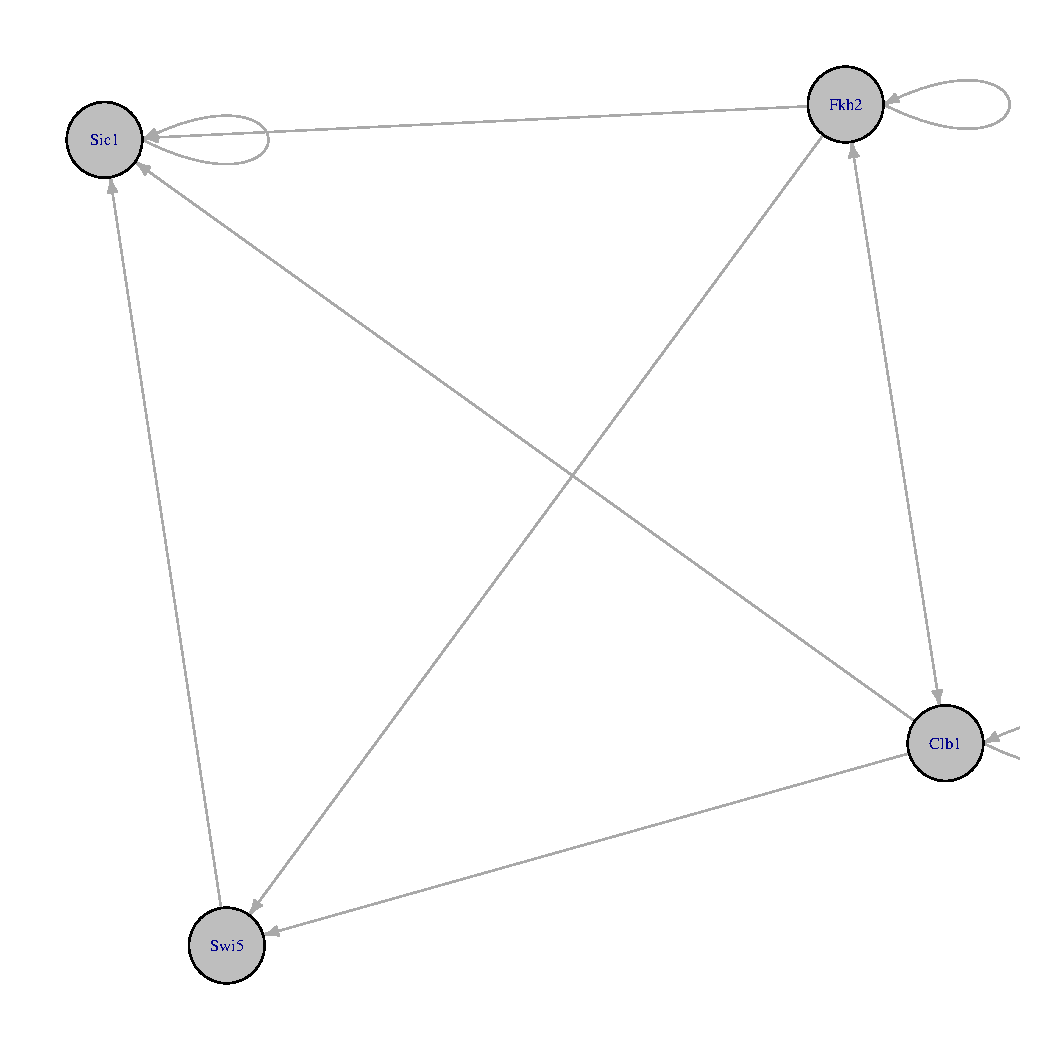
\includegraphics[width=0.5\linewidth]{wiring1}
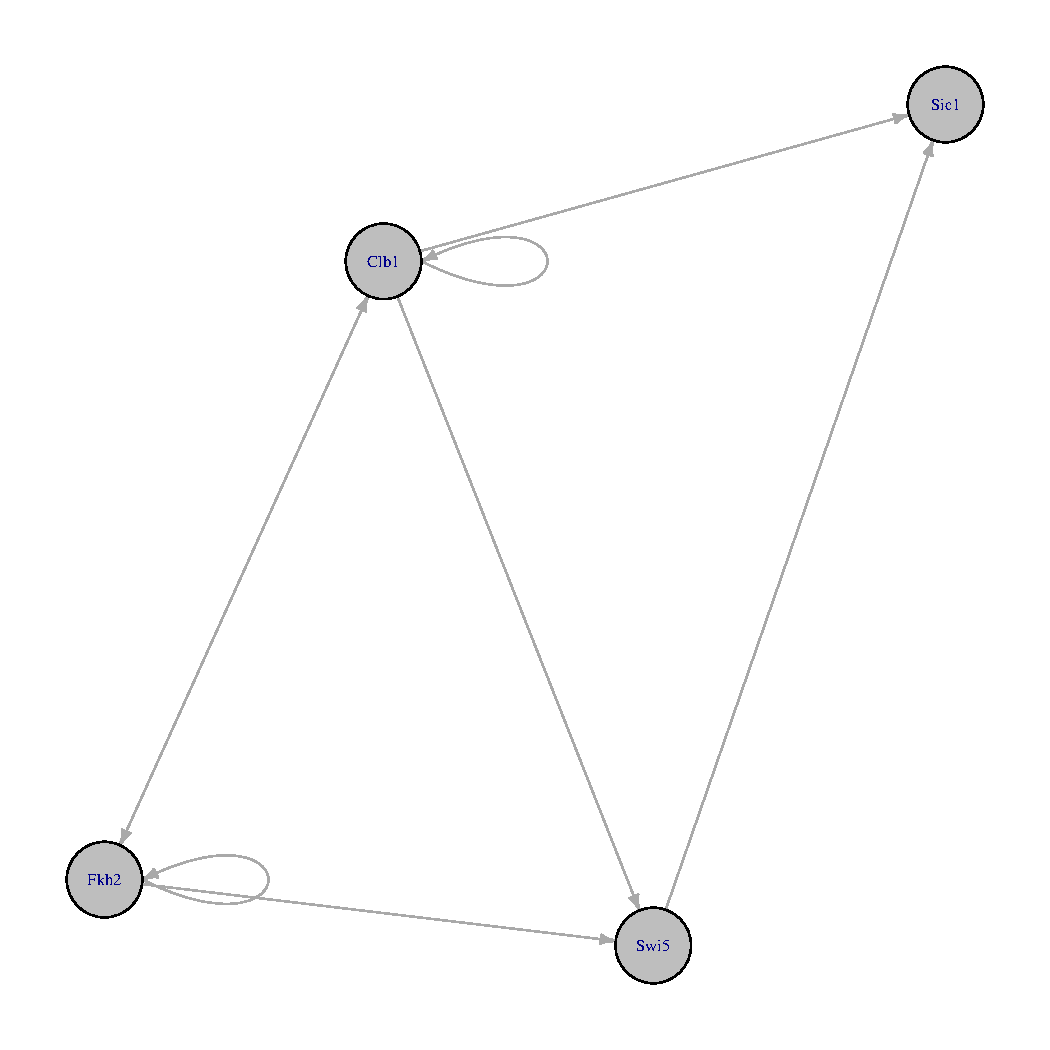
\includegraphics[width=0.5\linewidth]{wiring2}
\caption{The wiring graph of the reconstructed network without prior knowledge (top) and with the inclusion of prior knowledge (bottom). Each node of the graph represents one gene, and each arrow represents a gene dependency.}
\label{fig:wiring}
\end{figure}

A network that involved the same genes was examined by Kim et al. \cite{kim07}. When comparing the wiring graph of our reconstructed network with the reference network presented in Figure~2 of this paper, one observes a very high similarity between the two networks. However, the reconstructed network comprises too many links for the gene Sic1: The reference network does not contain a self-regulation of Sic1 or regulation of Sic1 by Fkh2. If it is known in advance that these regulations are not plausible, such prior knowledge can be supplied to the reconstruction algorithm:

\begin{knitrout}
\definecolor{shadecolor}{rgb}{0.969, 0.969, 0.969}\color{fgcolor}\begin{kframe}
\begin{alltt}
\hlstd{net} \hlkwb{<-} \hlkwd{reconstructNetwork}\hlstd{(binSeries}\hlopt{$}\hlstd{binarizedMeasurements,}
                          \hlkwc{method}\hlstd{=}\hlstr{"bestfit"}\hlstd{,}
                          \hlkwc{maxK}\hlstd{=}\hlnum{4}\hlstd{,}
                          \hlkwc{excludedDependencies} \hlstd{=} \hlkwd{list}\hlstd{(}\hlstr{"Sic1"} \hlstd{=} \hlkwd{c}\hlstd{(}\hlstr{"Sic1"}\hlstd{,} \hlstr{"Fkh2"}\hlstd{)))}
\end{alltt}
\end{kframe}
\end{knitrout}


The wiring of the reconstruction with prior knowledge is shown at the bottom of Figure~\ref{fig:wiring}. We can see that the two false links are now eliminated. Similar to \texttt{excludedDependencies}, there is also a parameter \texttt{requiredDependencies} that specifies dependencies that must be included in the network.

When \texttt{reconstructNetwork()} discovers multiple functions for a gene with the minimum error on the input data, it includes all of these functions as alternative functions with equal probability. Consequently, the function returns a \texttt{ProbabilisticBooleanNetwork} structure.

If you would like to obtain a \texttt{BooleanNetwork} object with only one function per gene from a probabilistic network, you can extract such a network by telling the software which of the functions you would like to use. This can be done by specifying the indices of the functions to extract:
\begin{knitrout}
\definecolor{shadecolor}{rgb}{0.969, 0.969, 0.969}\color{fgcolor}\begin{kframe}
\begin{alltt}
\hlstd{net} \hlkwb{<-} \hlkwd{reconstructNetwork}\hlstd{(binSeries}\hlopt{$}\hlstd{binarizedMeasurements,}
\hlkwc{method}\hlstd{=}\hlstr{"bestfit"}\hlstd{,} \hlkwc{maxK}\hlstd{=}\hlnum{4}\hlstd{)}
\hlstd{functionIndices} \hlkwb{<-} \hlkwd{c}\hlstd{(}\hlnum{1}\hlstd{,}\hlnum{2}\hlstd{,}\hlnum{3}\hlstd{,}\hlnum{2}\hlstd{)} \hlcom{#select function index for each regulatory component}
\hlstd{dontCareDefaults} \hlkwb{<-} \hlkwd{lapply}\hlstd{(}\hlkwd{seq_along}\hlstd{(net}\hlopt{$}\hlstd{interactions),} \hlkwa{function}\hlstd{(}\hlkwc{idx}\hlstd{)} \hlkwd{rep}\hlstd{(F,} \hlkwd{sum}\hlstd{(net}\hlopt{$}\hlstd{interactions[[idx]][[functionIndices[idx]]]}\hlopt{$}\hlstd{func} \hlopt{== -}\hlnum{1}\hlstd{)))} \hlcom{#determine number of don't care values for each selected function and set them to 0}
\hlkwd{names}\hlstd{(dontCareDefaults)} \hlkwb{<-} \hlstd{net}\hlopt{$}\hlstd{genes}
\hlstd{singleNet} \hlkwb{<-} \hlkwd{chooseNetwork}\hlstd{(net, functionIndices,} \hlkwc{dontCareValues} \hlstd{= dontCareDefaults)}
\end{alltt}
\end{kframe}
\end{knitrout}
In case of don't care values in reconstructed functions, it is possible to set them to 0 or 1 per default. The result is a Boolean network that is created by extracting the first function of gene Fkh2, the second function of genes Swi5 and Clb1, and the third function of gene Sic1 from the above probabilistic network:
\begin{knitrout}
\definecolor{shadecolor}{rgb}{0.969, 0.969, 0.969}\color{fgcolor}\begin{kframe}
\begin{alltt}
\hlstd{singleNet}
\end{alltt}
\begin{verbatim}
## Boolean network with 4 genes
## 
## Involved genes:
## Fkh2 Swi5 Sic1 Clb1
## 
## Transition functions:
## Fkh2 = <f(Clb1){01}>
## Swi5 = <f(Fkh2){01}>
## Sic1 = <f(Fkh2,Sic1){0001}>
## Clb1 = <f(Fkh2){01}>
\end{verbatim}
\end{kframe}
\end{knitrout}

\begin{sloppypar}
\texttt{BoolNet} also supports the generation of artificial time series from existing networks: The \texttt{generateTimeSeries()} function generates a set of time series from a network using random start states and optionally adds Gaussian noise.
\end{sloppypar}

\begin{knitrout}
\definecolor{shadecolor}{rgb}{0.969, 0.969, 0.969}\color{fgcolor}\begin{kframe}
\begin{alltt}
\hlstd{series} \hlkwb{<-} \hlkwd{generateTimeSeries}\hlstd{(cellcycle,}
                             \hlkwc{numSeries}\hlstd{=}\hlnum{100}\hlstd{,}
                             \hlkwc{numMeasurements}\hlstd{=}\hlnum{10}\hlstd{,}
                             \hlkwc{noiseLevel}\hlstd{=}\hlnum{0.1}\hlstd{)}
\end{alltt}
\end{kframe}
\end{knitrout}
generates a list of 100 time series by calculating 10 consecutive transitions from 100 randomly chosen network states in the mammalian cell cycle network. The series are subject to Gaussian noise with a standard deviation of 0.1, such that the result is a list of real-valued matrices.

We can now binarize these simulated measurements and try to reconstruct the original network:
\begin{knitrout}
\definecolor{shadecolor}{rgb}{0.969, 0.969, 0.969}\color{fgcolor}\begin{kframe}
\begin{alltt}
\hlstd{binSeries} \hlkwb{<-} \hlkwd{binarizeTimeSeries}\hlstd{(series,} \hlkwc{method}\hlstd{=}\hlstr{"kmeans"}\hlstd{)}
\hlstd{net} \hlkwb{<-} \hlkwd{reconstructNetwork}\hlstd{(binSeries}\hlopt{$}\hlstd{binarizedMeasurements,} \hlkwc{method}\hlstd{=}\hlstr{"bestfit"}\hlstd{)}
\hlstd{net}
\end{alltt}
\begin{verbatim}
## Probabilistic Boolean network with 10 genes
## 
## Involved genes:
## CycD Rb E2F CycE CycA p27 Cdc20 Cdh1 UbcH10 CycB
## 
## Transition functions:
## 
## Alternative transition functions for gene CycD:
## CycD = <f(CycD){01}> (error: 0)
## 
## Alternative transition functions for gene Rb:
## Rb = <f(CycD,CycE,p27,CycB){1010001000000000}> (error: 0)
## 
## Alternative transition functions for gene E2F:
## E2F = <f(Rb,CycA,p27,CycB){1010001000000000}> (error: 0)
## 
## Alternative transition functions for gene CycE:
## CycE = <f(Rb,E2F){0100}> (error: 0)
## 
## Alternative transition functions for gene CycA:
## CycA = <f(Rb,E2F,Cdc20,Cdh1,UbcH10){11000000111000000000000000000000}> (error: 5)
## CycA = <f(Rb,E2F,CycA,Cdc20,UbcH10){00001100100011000000000*00000*00}> (error: 5)
## 
## Alternative transition functions for gene p27:
## p27 = <f(CycD,CycE,CycA,p27,CycB){1010*010001000000000*00000000000}> (error: 0)
## 
## Alternative transition functions for gene Cdc20:
## Cdc20 = <f(CycB){01}> (error: 0)
## 
## Alternative transition functions for gene Cdh1:
## Cdh1 = <f(CycA,p27,Cdc20,CycB){1011101100111011}> (error: 0)
## 
## Alternative transition functions for gene UbcH10:
## UbcH10 = <f(CycA,Cdc20,Cdh1,UbcH10,CycB){11110001111100111111001111*10011}> (error: 0)
## 
## Alternative transition functions for gene CycB:
## CycB = <f(Cdc20,Cdh1){1000}> (error: 0)
\end{verbatim}
\end{kframe}
\end{knitrout}

Obviously, the number of generated time series is still to small to reconstruct the network unambiguously. However, the result comes close to the original network. We see that the functions of the network are not fully specified: At some positions, there are asterisks (\texttt{*}) denoting a \emph{don't care} value. This means that functions with a 0 and a 1 at this position match the time series equally well. That is, a partially defined function with $m$ asterisks corresponds to $2^m$ fully defined Boolean functions. It is also possible to generate these fully defined functions instead of the partially defined function by setting the parameter \texttt{returnPBN} to true (which was the behaviour prior to \texttt{BoolNet} version 2.0). For many \emph{don't care} values, this may consume a high amount of memory and computation time. 

\texttt{generateTimeSeries()} can also generate time series with artificial knock-outs and overexpressions:













































































































































































